\documentclass[11pt]{article}
\usepackage{amsmath, amsthm, amssymb, pdfpages} 
\usepackage{fullpage}
\usepackage{hyperref}
\usepackage{graphicx}
\usepackage[capitalize]{cleveref}
\usepackage{appendix}

% next three for UTF8 to work (for non-ASCII names to work without awkward codes)
\usepackage[T1]{fontenc}
\usepackage{textcomp}
\usepackage[utf8]{inputenc}

% import biblatex with prefered settings
% loads biblatex with all the nice standard options that John determined some time ago!
% this version uses a ``Harvard'' style (first author last name, year in parentheses).
% also loads xpatch

% biblatex
% harvard style
\usepackage[style=authoryear,natbib,maxcitenames=2,doi=true,isbn=false,url=false,backend=bibtex]{biblatex}
% numeric style
%% \usepackage[style=numeric-comp,sorting=none,giveninits=true,
%%                      doi=false,isbn=false,url=false,backend=bibtex]{biblatex}
% remove "In: " before journal title
\renewbibmacro{in:}{}
% remove language
\AtEveryBibitem{\clearlist{language}}
% remove month
\AtEveryBibitem{\clearfield{month}}
% and also notes
\AtEveryBibitem{\clearfield{note}}
% remove dots between volume and issue
\usepackage{xpatch}
\xpatchbibmacro{volume+number+eid}{%
  \setunit*{\adddot}%
}{%
}{}{}
% put issue in parentheses
\DeclareFieldFormat[article]{number}{\mkbibparens{#1}}


\bibliography{zotero} % biblatex wants this in the preamble...

% copied from PCA-GWAS paper
\newcommand{\rmsd}{\text{SRMSD}_p}
\newcommand{\auc}{\text{AUC}_\text{PR}}

\usepackage{kinshipsymbols}
% % copy of \Fst from package `kinshipsymbols`

% some more definitions
\newcommand{\kinMat}[1][T]{%
  \ensuremath{%
    \mathbf{\Phi}^{#1}
  }%
  \xspace%
}%
\newcommand{\kinMatPrime}{%
  \ensuremath{%
    \mathbf{\Phi}^{T\prime}
  }%
  \xspace%
}%
\newcommand{\kinMatEstNamed}[1]{%
  \ensuremath{%
    \mathbf{\hat{\Phi}}^{T,\text{#1}}
  }%
  \xspace%
}%

% double line spacing (PLoS wants this)
\usepackage{setspace}
\doublespacing

% cool automatic supplemental figures/tables!
% http://bytesizebio.net/2013/03/11/adding-supplementary-tables-and-figures-in-latex/
% with some additions
\newcommand{\beginsupplement}{%
  \setcounter{table}{0}
  \renewcommand{\thetable}{S\arabic{table}}%
  \setcounter{figure}{0}
  \renewcommand{\thefigure}{S\arabic{figure}}%
  \setcounter{section}{0}
  \renewcommand{\thesection}{S\arabic{section}}%
  \setcounter{equation}{0}
  \renewcommand{\theequation}{S\arabic{equation}}%
  \setcounter{page}{1}
  \renewcommand{\thepage}{S\arabic{page}}%
}


\title{\Large \textbf{Genetic association models are robust to common population kinship estimation biases}}
\author{Zhuoran Hou$^1$, Alejandro Ochoa$^{1,2,*}$}
\date{}

\begin{document}
\maketitle

\noindent
$^1$ Department of Biostatistics and Bioinformatics, Duke University, Durham, NC 27705, USA \\
$^2$ Duke Center for Statistical Genetics and Genomics, Duke University, Durham, NC 27705, USA \\
$^*$ Corresponding author: \texttt{alejandro.ochoa@duke.edu}


% 2,300 characters for ASHG submission
% current 230 words, 1588 characters (including double spaces)
\begin{abstract}
  Common genetic association studies for structured populations, including Principal Component Analysis (PCA) and Linear Mixed-effects Models (LMM), model the correlation structure between individuals using population kinship matrices, also known as Genetic Relatedness Matrices or ``GRMs''.
  However, the most common kinship estimators can have severe biases that were only recently characterized.
  Here we characterize the effect of these kinship biases on genetic association.
  We employ a large simulated admixed family and genotypes from the 1000 Genomes Project, both with simulated traits, to evaluate a variety of kinship matrices (every bias type has two locus weight types, and their theoretical limits for the simulation).
  Remarkably, we find nearly equal association statistics and performance for kinship matrices of different bias types (when all other features are matched).
  These empirical observations lead us to hypothesize that these association tests are invariant to these kinship biases, which using linear algebra we prove holds exactly for LMM and approximately for PCA.
  Our constructive proof shows that the intercept and relatedness (PCs in PCA, random effect in LMM) coefficients compensate for the kinship bias, so the result extends to generalized linear models as long as those coefficients are present and are nuisance parameters.
  A corollary of our results is that association testing is also invariant to changing the ancestral population used to determine the kinship matrix.
  Overall, we find that existing association studies are robust to kinship estimation bias, and our calculations may help improve association methods by taking advantage of this unexpected robustness, as well as help determine the effects of kinship bias in related problems.
\end{abstract}

\section{Introduction}

% GWAS, LMM and PCA
The goal of genetic association is to detect loci that are related to a specific trait, either causally or by proximity to causal loci.
When applied to structured populations with admixed individuals, multiethnic cohorts, or close relatives, controlling for relatedness is crucial to avoid spurious associations and loss of power \citep{devlin_genomic_1999, voight_confounding_2005, astle_population_2009, yao_limitations_2022}.
The most popular association models for structured populations are Linear Mixed-effects Models (LMM) and Principal Component Analysis (PCA), which are closely related except LMM is capable of modeling high-dimensional structures whereas PCA is strictly a low-dimensional model \citep{astle_population_2009, hoffman_correcting_2013, yao_limitations_2022}.

% Kinship in models
Various association models, including both PCA and LMM, parametrize relatedness using kinship matrices, also known as Genetic Relatedness Matrices or ``GRMs''.
Kinship coefficients are well suited for this task since they model the covariance structure of genotypes \citep{malecot_mathematiques_1948, jacquard_structures_1970}.
Kinship is often encountered in family studies, where they reflect recent relatedness and can be calculated from pedigrees \citep{wright_coefficients_1922, emik_systematic_1949, garcia-cortes_novel_2015}.
However, as kinship is defined as a probability of identity by descent, it may also capture ancient population relatedness \citep{malecot_mathematiques_1948, astle_population_2009}, and common non-parametric kinship estimators from genotypes indeed include population structure in their estimates \citep{ochoa_estimating_2021}.
In LMMs, the kinship matrix is an explicit parameter determining the random effect covariance structure \citep{xie_combining_1998,yu_unified_2006, aulchenko_genomewide_2007, astle_population_2009, kang_efficient_2008, kang_variance_2010, zhou_genome-wide_2012, yang_advantages_2014, loh_efficient_2015, sul_population_2018}.
In PCA, the principal components (PCs) are in practice the eigenvectors of an empirical genetic covariance matrix that is equivalent to the most common kinship estimator \citep{price_principal_2006, astle_population_2009, hoffman_correcting_2013, yao_limitations_2022}.

% kinship estimators
Although several kinship estimators have been used with LMMs in the past, work from the last 15 years has converged on what we call the ``standard'' kinship estimator, which is the same estimator used in PCA and other related models \citep{price_principal_2006, astle_population_2009, rakovski_kinship-based_2009, thornton_roadtrips:_2010, yang_common_2010, yang_gcta:_2011, zhou_genome-wide_2012, speed_improved_2012, yang_advantages_2014, speed_relatedness_2015, loh_efficient_2015, wang_efficient_2017, sul_population_2018}.
The impetus of our work is the recent characterization of a complex bias for this standard estimator, which varies for every pair of individuals \citep{weir_unified_2017, ochoa_estimating_2021}.
This recent work also produced two new kinship estimators, which we are interested in characterizing in the context of association.
The Weir-Goudet (WG) estimator constitutes a key improvement in that it has a uniformly downward bias \citep{weir_unified_2017, ochoa_estimating_2021}.
Lastly, the popkin estimator is the only unbiased estimator under arbitrary relatedness \citep{ochoa_estimating_2021}.
To the best of our knowledge, the new WG and popkin estimators have not been used in association studies before, but represent potential improvements over the use of the standard estimator for association.

% MOR vs ROM
One potential confounder when comparing the above kinship estimators is that the standard estimator upweights rare variants in a formulation previously called ``mean-of-ratios'' (MOR), whereas WG and popkin do not, instead following a ``ratio-of-means'' (ROM) estimation strategy \citep{bhatia_estimating_2013, ochoa_estimating_2021}.
Recent work also formulated a ROM version of the standard estimator, which has a more predictable bias than the widely used MOR version \citep{ochoa_estimating_2021}.
Following a locus weight formulation that allows the standard estimator to weigh loci in both ways \citep{wang_efficient_2017}, here we generalized the popkin and WG estimators to have both MOR and ROM versions as well, in order to test for the effect of estimator bias without confounding by locus weighing strategy.

% This work summary
In this work, we originally hypothesized that kinship estimation bias would affect association testing.
We perform evaluations using an admixed family simulation \citep{yao_limitations_2022} as well as real genotypes from the 1000 Genomes project \citep{the_1000_genomes_project_consortium_map_2010, 1000_genomes_project_consortium_integrated_2012, fairley_international_2020}, in both cases with simulated traits in order to characterize type I error control and power using robust statistics.
Surprisingly, we found that both LMM and PCA association are robust to kinship estimation bias to an extent that most association statistics are invariant to these biases.
Lastly, we theoretically characterize the conditions under which these kinship biases result in invariant association statistics, which encompass changing ancestral population in the kinship matrix too.
Overall, we found that long-used association approaches are robust to the most common kinship estimation biases, and developed theoretical results that may help improve association and related approaches such as heritability estimation.


\section{Methods}

\subsection{Genetic model}

The following genetic model justifies the use of kinship matrices in association studies, and is the basis of all kinship estimation bias calculations that our theoretical work depends upon.

Suppose there are $m$ biallelic loci and $n$ diploid individuals.
The genotype $\xij \in \{0,1,2\}$ at a locus $i$ of individual $j$ is encoded as the number of reference alleles, for a preselected but otherwise arbitrary reference allele per locus.
These genotypes can be treated as random variables structured according to relatedness.
If $T$ is the ancestral population on which allele frequencies are being conditioned, \kt is the kinship coefficient of two individuals $j$ and $k$, and \pit is the ancestral allele frequency at locus $i$, then under the kinship model \citep{ochoa_estimating_2021} the expectation and covariance are given by
\begin{align*}
  \E \left[ \mathbf{x}_i \middle| T \right]
  =
    2 \pit \mathbf{1}
  ,
  \quad\quad
  \Cov \left(\mathbf{x}_i \middle| T \right)
  =
    4 \pit \left( 1 - \pit \right) \kinMat
    ,
\end{align*}
where $\mathbf{x}_i = (\xij)$ is the length-$n$ column vector of genotypes at locus $i$, $\kinMat = (\kt)$ is the $n \times n$ kinship matrix, and $\mathbf{1}$ is a length-$n$ column vector of ones.
Both \kinMat and \pit are parameters that depend on the choice of ancestral population, for which the Most Recent Common Ancestor (MRCA) population is the most sensible choice \citep{ochoa_estimating_2021}.
However, one of the results of this work is proof that the choice of ancestral population does not affect association testing.

\subsection{Kinship estimators}

Each subsection below corresponds to a kinship estimator bias type: Popkin is unbiased, while Standard and WG have different bias functions (defined shortly).
Each estimator bias type has two locus-weight versions, some introduced in this work, called \textit{ratio-of-means} (ROM) and \textit{mean-of-ratios} (MOR), a terminology that follows previous convention for these and related estimators \citep{bhatia_estimating_2013, ochoa_estimating_2021}.
Only ROM estimators have closed-form limits.
Below
$
\pith
=
\frac{1}{2n} \mathbf{x}_i^\intercal \mathbf{1}
$
is the standard ancestral allele frequency estimator,
where the $\intercal$ superscript denotes matrix transposition (do not confuse with ancestral population superscript $T$),
and
$\kinMatEstNamed{name} = (\ktHatNamed{name})$
relates the scalar and matrix formulas of each named kinship estimator.

\subsubsection{Popkin estimator}

The popkin (population kinship) estimator \citep{ochoa_estimating_2021}, generalized here to include locus weights $w_i$, is given by
\begin{equation}
  \label{eq:popkin}
  \ktHatNamed{popkin}
  =
  1 - \frac{\Ajk}{\AMinHat}
  , \quad\quad
  \Ajk
  =
  \frac{1}{m} \sum_{i=1}^m w_i ( (\xij-1)(\xij[k]-1) - 1 )
  ,
\end{equation}
where in this work $\AMinHat = \min_{j \ne k} \Ajk$, and $w_i$ must be positive but need not add to 1.
We consider two broad forms for this estimator.
The original ROM estimator has $w_i = 1$ and has an unbiased almost sure limit as the number of loci $m$ go to infinity,
$$
\kinMatEstNamed{popkin-ROM} \toas \kinMat,
% \ktHatNamed{popkin-ROM} \toas \kt,
$$
under the assumption that the true minimum kinship is zero.
The MOR version, introduced here, upweighs rare variants by using $w_i = \left( \pith \left( 1 - \pith \right) \right)^{-1}$; although it has no closed-form limit, it is approximately unbiased as well (\cref{sec:popkin_w_justif}) and it is connected to the most common estimator, Standard MOR (\cref{sec:conn_popkin_std}). 
The use of locus weights here is inspired by previous calculations relating the standard ROM and MOR estimators \citep{wang_efficient_2017}.

\subsubsection{Standard estimator}

The ROM and MOR versions of the standard kinship estimator are, respectively,
\begin{align}
  \label{eq:kinship_std_rom}
  \ktHatNamed{std-ROM}
  &=
    \frac{
    \sum\limits_{i=1}^m \left( \xij - 2 \pith \right) \left( \xij[k] - 2 \pith \right)
    }{
    \sum\limits_{i=1}^m 4 \pith \left( 1-\pith \right)
    }
    , \\
  \label{eq:kinship_std_mor}
  \ktHatNamed{std-MOR}
  &=
    \frac{1}{m} \sum\limits_{i=1}^m \frac{\left( \xij - 2 \pith \right) \left( \xij[k] - 2 \pith \right)}{4 \pith \left( 1-\pith \right)}
    .
\end{align}
The ROM estimator has a biased limit, which is a function of the true kinship matrix \citep{ochoa_estimating_2021}:
\begin{equation}
  \label{eq:kinship_std_lim}
  \kinMatEstNamed{std-ROM}
  \toas
  F^\text{std} \left( \kinMat \right)
  =
  \frac{1}{1 - \bar{\varphi}^T}
  \left(
    \kinMat
    + \bar{\varphi}^T \mathbf{J}
    - \boldsymbol{\varphi}^T \mathbf{1}^\intercal 
    - \mathbf{1} \left( \boldsymbol{\varphi}^T \right)^\intercal 
  \right)
  ,
\end{equation}
where
$\mathbf{J} = \mathbf{1} \mathbf{1}^\intercal$ is the $n \times n$ matrix of ones,
$\boldsymbol{\varphi}^T = \frac{1}{n} \kinMat \mathbf{1}$ is a length-$n$ vector of per-row mean kinship values, and
$\bar{\varphi}^T = \frac{1}{n^2} \mathbf{1}^\intercal \kinMat \mathbf{1}$ is the scalar overall mean kinship.
The MOR estimator does not have closed-form limit, but it is well approximated by \cref{eq:kinship_std_lim} in practice, especially when loci with small minor allele frequencies are excluded prior to calculating this estimate.
In \cref{sec:conn_popkin_std} we prove that the two standard estimators are functions of the corresponding popkin estimators, given by the bias function $F^\text{std}$:
\begin{align*}
  \kinMatEstNamed{std-ROM}
  &=
    F^\text{std} \left( \kinMatEstNamed{popkin-ROM} \right)
    , \\
  \kinMatEstNamed{std-MOR}
  &=
    F^\text{std} \left( \kinMatEstNamed{popkin-MOR} \right)
    .
\end{align*}

\subsubsection{Weir-Goudet estimator}

The ROM version of the Weir-Goudet (WG) kinship estimator is given by \citep{weir_unified_2017, ochoa_estimating_2021}
\begin{equation}
  \label{eq:wg}
  \ktHatNamed{WG-ROM}
  =
  1 - \frac{\Ajk}{\AAvgHat}
  , \quad\quad
  \AAvgHat
  =
  \frac{2}{n(n-1)}
  \sum_{j=2}^n
  \sum_{k=1}^{j-1}
    \Ajk
    ,
\end{equation}
where \Ajk is as in \cref{eq:popkin}.
Its biased limit is also a function of the true kinship matrix:
\begin{equation}
  \label{eq:wg_lim}
  \kinMatEstNamed{WG-ROM}
  \toas
  F^\text{WG} \left( \kinMat \right)
  =
  \frac{1}{1 - \tilde{\varphi}^T}
  \left( \kinMat - \tilde{\varphi}^T \mathbf{J} \right)
  ,
\end{equation}
where $\tilde{\varphi}^T$ is the mean kinship excluding the matrix diagonal:
\begin{equation}
  \label{eq:wg_tilde}
  \begin{split}
    \tilde{\varphi}^T
    &=
    \frac{2}{n(n-1)}
    \sum_{j=2}^n
    \sum_{k=1}^{j-1}
    \kt
    .
  \end{split}
\end{equation}
In \cref{sec:wg_posdef} we prove that $F^\text{WG} \left( \kinMat \right)$ is positive definite if \kinMat also is.
In \cref{sec:mean_kinship_ineqs} we prove that
$$
0 \le \tilde{\varphi}^T \le \bar{\varphi}^T \le \bar{\delta}^T \le 1,
$$
where $\bar{\delta}^T = \frac{1}{n} \sum_{j=1}^n \kt[j]$, and equalities are achieved if and only if all kinship values are equal.
Since the WG-ROM estimator closely resembles the popkin estimator in \cref{eq:popkin}, it follows more straightforwardly that they are related by the bias function $F^\text{WG}$, while WG-MOR is introduced here and defined by the below formula:
\begin{align*}
  \kinMatEstNamed{WG-ROM}
  &=
    F^\text{WG} \left( \kinMatEstNamed{popkin-ROM} \right)
    , \\
  \kinMatEstNamed{WG-MOR}
  &=
    F^\text{WG} \left( \kinMatEstNamed{popkin-MOR} \right)
  .
\end{align*}

\subsection{Association models}

LMM and PCA are closely-related association models \citep{astle_population_2009, hoffman_correcting_2013, yao_limitations_2022}:
\begin{align}
  \label{eq:lmm_gwas}
  \text{LMM:}\quad
  \mathbf{y}
  &=
    \mathbf{1} \alpha + \mathbf{x}_i \beta_i + \mathbf{s} + \boldsymbol{\epsilon}
    , \\
  \label{eq:lmm_rand_eff}
  \mathbf{s}
  &\sim
    \text{Normal} \left( \mathbf{0}, 2 \sigma^2 \kinMat \right), \\
  \label{eq:pca_gwas}
  \text{PCA:}\quad
  \mathbf{y}
  &=
    \mathbf{1} \alpha + \mathbf{x}_i \beta_i + \mathbf{U}_d \boldsymbol{\gamma}_d + \boldsymbol{\epsilon}
    , \\
  \label{eq:kin_evd}
  \kinMat
  &=
    \mathbf{U} \mathbf{\Lambda} \mathbf{U}^\intercal
    ,
\end{align}
where
$\mathbf{y}$ is a length-$n$ vector of continuous trait values,
$\alpha$ is the intercept coefficient,
$\beta_i$ is the genetic effect (association) coefficient of locus $i$,
$\mathbf{s}$ is the (genetic) random effect,
$\sigma^2$ is the random effect variance factor,
$\mathbf{U}_d$ is the $n \times d$ matrix of top-$d$ eigenvectors of \kinMat (often refered to as ``principal components'' in genetics),
$\boldsymbol{\gamma}_d$ is a length-$d$ vector of coefficients for each eigenvector,
$\boldsymbol{\epsilon} \sim \text{Normal}(\mathbf{0}, \sigma^2_\epsilon \mathbf{I})$ are random independent residuals,
and $\mathbf{I}$ is the $n \times n$ identity matrix.
Furthermore, \cref{eq:kin_evd} is the complete eigendecomposition of \kinMat,
where $\mathbf{U}$ is the $n \times n$ matrix of eigenvectors, and
$\mathbf{\Lambda}$ is the $n \times n$ diagonal matrix of eigenvalues.
As $\mathbf{s}$ and $\mathbf{U}_d$ play analogous roles in modeling the effect of relatedness in LMM and PCA, respectively, we refer to them jointly as ``relatedness'' effects, and $\sigma$ and $\boldsymbol{\gamma}_d$ as their respective coefficients.

\subsection{Simulations}

\subsubsection{Admixed family genotype simulation}

An admixed family was simulated following previous work \citep{yao_limitations_2022}, except here only $K=3$ ancestries were simulated and $F_{ST}=0.3$ for the admixed individuals, which more closely resembles the parameters of recently-admixed individuals such as Hispanics and African-Americans.
Briefly, our admixture model first simulates $n=1000$ founder individuals with the number of loci $m=100,000$.
Random ancestral allele frequencies \pit, subpopulation allele frequencies $p_i^{S_u}$, individual-specific allele frequencies $\pi_{ij}$, and genotypes \xij are drawn from this hierarchical model:
\begin{align*}
  \pit
  &\sim
    \text{Uniform}( 0.01, 0.5 )
    , \\
  p_i^{S_u} | \pit
  &\sim
    \text{Beta} \left(
    \pit \left( \frac{1}{ \ft[S_u] } - 1 \right),
    \left( 1 - \pit \right) \left( \frac{1}{ \ft[S_u] } - 1 \right)
    \right)
    , \\
  \pi_{ij}
  &=
    \sum_{u = 1}^K q_{ju} p_i^{S_u}
    , \\
  \xij | \pi_{ij}
  &\sim
    \text{Binomial}(2, \pi_{ij})
    ,
\end{align*}
where this Beta is the Balding-Nichols distribution \citep{balding_method_1995} with mean \pit and variance $\pit \left( 1 - \pit \right) \ft[S_u]$.
This is implemented in the R package \texttt{bnpsd}.

We also include family structure in the simulation. 20 generations are generated iteratively. To preserve admixture structure mentioned above, individuals in the first generation ($n=1000$) are ordered by 1D geography, locally unrelated and randomly assigned sex. 
From the next generation, individuals are paired iteratively: randomly choosing males from the pool and pairing them with the nearest available female with local kinship $<1/4^3$ until no available males or females. Family sizes are drawn randomly ensuring every family has at least one child. Children are reordered by the average coordinates of their parents, their sex are assigned randomly, and their alleles are drawn from parents independently per locus. The simulation is implemented in the R package \texttt{simfam}.

\subsubsection{Trait simulation algorithm}

Given an $m \times n$ genotype matrix $\mathbf{X} = (\mathbf{x}_i^\intercal)$, traits are simulated from
$$
\mathbf{y}
=
\mathbf{1} \alpha + \mathbf{X}^\intercal \boldsymbol{\beta} + \boldsymbol{\epsilon}
, \quad\quad
\boldsymbol{\epsilon} \sim \text{Normal}(\mathbf{0}, (1 - h^2) \mathbf{I})
.
$$
Given a desired number of causal loci $m_1 = n/10$ and heritability $h^2=0.8$, the goal is to choose causal coefficients $\boldsymbol{\beta}$ and the intercept $\alpha$ that result in zero mean and the desired trait heritability.
Here, we use the ``fixed effect sizes'' trait simulation model described in \citep{yao_limitations_2022}.
Briefly, first $m_1$ causal loci are randomly selected, and for these steps only $\mathbf{X}$ is subset to these loci and reindexed.
For known \pit, causal coefficients are constructed as:
$$
\beta_i = \sqrt{ \frac{h^2}{ 2 m_1 v_i^T } },
$$
where
$
v_i^T
=
\pit \left( 1 - \pit \right)
;
$
for unknown \pit,  $v_i^T$ is replaced by the unbiased estimate
$
\hat{v}_i^T
=
\pith \left( 1 - \pith \right) / \left( 1 - \bar{\varphi}^T \right)
,
$
where $\bar{\varphi}^T$ is the mean kinship estimated from \texttt{popkin}.
Coefficients are made negative randomly with probability 0.5.
For known \pit, we obtain the desired zero trait mean with
$
\alpha 
=
- 2 \left( \mathbf{p}^T \right)^\intercal \boldsymbol{\beta}
,
$
where here $\mathbf{p}^T = (\pit)$ contains causal loci only.
When \pit are unknown, to avoid covariance distortions, the intercept coefficient is constructed as
\begin{align*}
  \alpha 
  =
  - 2 \hat{\bar{p}}^T \mathbf{1}_{m_1}^\intercal \boldsymbol{\beta}
  , \quad\quad
  \hat{\bar{p}}^T
  =
  \frac{1}{m_1} \mathbf{1}_{m_1}^\intercal \mathbf{\hat{p}}^T
  ,
\end{align*}
where $\mathbf{1}_{m_1}$ is a length-$m_1$ column vector of ones.

\subsection{Real genotype data processing}

To evaluate different kinship estimators on a real dataset, we use the high-coverage NYGC version of the 1000 Genomes Project \citep{fairley_international_2020}, which were processed as before \citep{yao_limitations_2022}.
Briefly, using \texttt{plink2} \citep{chang_second-generation_2015} we kept only autosomal biallelic SNP loci with filter ``PASS'', LD-pruned with parameters ``\texttt{-{}-indep-pairwise 1000kb 0.3}'' to remove loci that have a greater than 0.3 correlation coefficient with other loci within 1000kb, and lastly remove loci with $\text{MAF} < 0.01$.
The resulting data has $m=1,111,266$ loci and $n=2,504$ individuals.
Traits were simulated for this dataset with $m_1 = n/10 = 250$ causal loci.

\subsection{Evaluation of performance}

$\auc$ and $\rmsd$ are used to evaluate approaches as before \citep{yao_limitations_2022}.
Briefly, $\rmsd$ (Signed Root Mean Square Deviation) is used to measure the difference between the observed null p-value quantiles and the expected uniform quantiles (p-values of continuous test statistics follow a uniform distribution under the null):
$$
\rmsd
=
\text{sgn}(u_\text{median} - p_\text{median} ) \sqrt{ \frac{1}{m_0} \sum_{i = 1}^{m_0} \left( u_i - p_{(i)} \right)^2 },
$$
where
$m_0 = m - m_1$ is the number of null (non-causal) loci,
$i$ indexes null loci only,
$p_{(i)}$ is the $i$th ordered null p-value,
$u_i = ( i - 0.5 ) / m_0$ is its expectation,
$p_\text{median}$ is the median observed null p-value,
$u_\text{median} = \frac{1}{2}$ is its expectation,
and $\text{sgn}$ is the sign function (1 if $u_\text{median} \ge p_\text{median}$, -1 otherwise).
$\rmsd = 0$ corresponds to calibrated p-values, $\rmsd > 0$ indicate anti-conservative p-values, and $\rmsd < 0$ are conservative p-values.

$\auc$ (Area Under the Precision and Recall Curve) is a binary classification measure calculated from the total numbers of true positives (TP), false positives (FP) and false negatives (FN) at some threshold or parameter $t$:
\begin{align*}
  \text{Precision}(t)
  &=
    \frac{ \text{TP}(t) }{ \text{TP}(t) + \text{FP}(t) }
    , \\
  \text{Recall}(t)
  &=
    \frac{ \text{TP}(t) }{ \text{TP}(t) + \text{FN}(t) }
    ,
\end{align*}
followed by calculating the area under the curve traced as $t$ varies recall from zero to one.
Higher $\auc$ is better, with best performance at $\auc = 1$ for a perfect classifier, while worst performance at $\auc = \frac{m_1}{m}$ (overall proportion of causal loci) is for random classifiers.



\subsection{Software}

% kinship-specific software
Popkin estimates were calculated with the \texttt{popkin} R package.
Standard kinship estimates were calculated with GCTA (version 1.93.2beta).
All other estimators and limits were calculated using the \texttt{popkinsuppl} R package.
PCs were calculated with the \texttt{eigen} function of R.

% association-specific software
GCTA was used to run all LMM associations \citep{yang_gcta:_2011, yang_advantages_2014}. We pass $2 \kinMat$ for all kinship matrices tested (the same scale as its own kinship estimate).
PCA association is performed with \texttt{plink2} \citep{chang_second-generation_2015}.
We used $r=k-1=2$ for the admixed family simulations, and $r=10$ for 1000 Genomes.

\section{Results}

% path for figures
\graphicspath{ {../data/} }

\subsection{Empirical analysis using admixed family simulation}

% overview of sim results
To quantify the effect of kinship estimation bias, we simulated genotypes and traits, and calculated association p-values using a factorial design that tests all kinship matrix (3 bias types, times two locus weight versions and one limit) and association model (PCA and LMM) combinations.
We first simulated an admixed population with $K=3$ ancestries, then simulated a 20-generation random pedigree from the admixed population as founders.
This high-dimensional admixed family scenario yields a large difference in performance between PCA and LMM \citep{yao_limitations_2022}.

\begin{figure}[bp!]
  \centering
  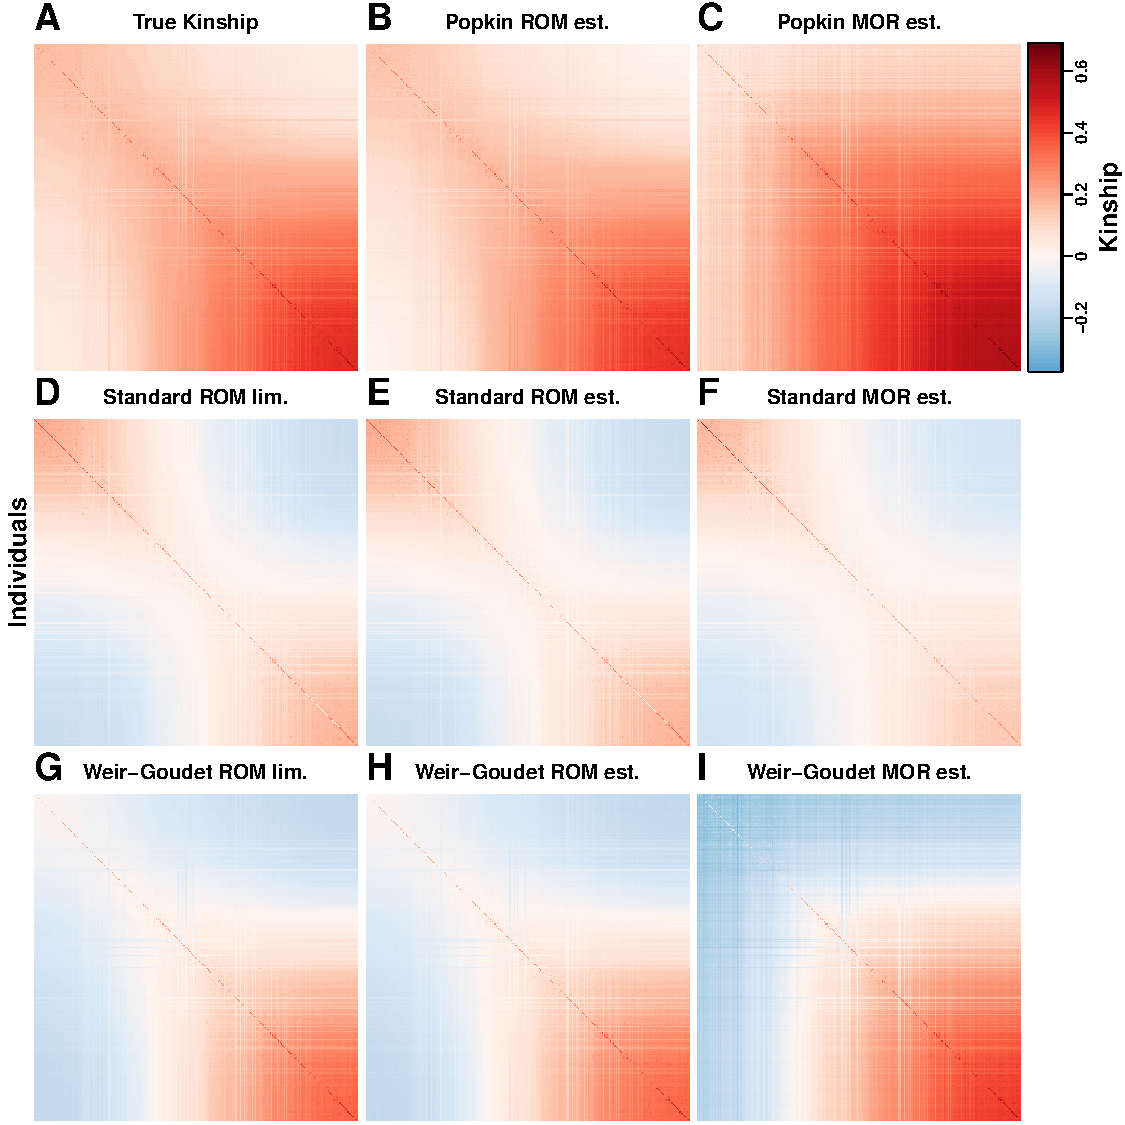
\includegraphics[height=0.8\textheight]{sim-admix-n1000-m100000-k3-f0.3-s0.5-mc100-h0.8-g20-fes/kinship.pdf}
  \caption{
    {\bf Kinship estimates and limits on the admixed family simulation.}
    Each panel shows a kinship matrix as a heatmap, with each of the $n=1000$ individuals along both x and y axes, color represents kinship: positive estimates in red, negative in blue.
    Diagonal contains inbreeding estimates.
    Each estimator bias type (Popkin, Standard, and Weir-Goudet; rows) has three matrices (columns): two locus-weight versions (ROM (ratio of means) and MOR (mean of ratios)) and limit of ROM.
  }
  \label{fig:kinship_sim}
\end{figure}

% kinship matrices
Kinship estimates and available limits on this simulation are shown in \cref{fig:kinship_sim}.
The true kinship matrix shows the family relatedness as high values concentrated near the diagonal and the ancestry-driven population structure as the broad patterns off-diagonal.
Only Popkin ROM is unbiased, while popkin MOR has a slight upward bias that varies across the matrix (\cref{fig:popkin-rom-mor}A).
In contrast, the Standard and Weir-Goudet (WG) estimates have large downward biases overall, resulting in abundant negative values; for Standard these biases vary for every pair of individuals whereas for WG they are uniform.

\begin{figure}[bp!]
  \centering
  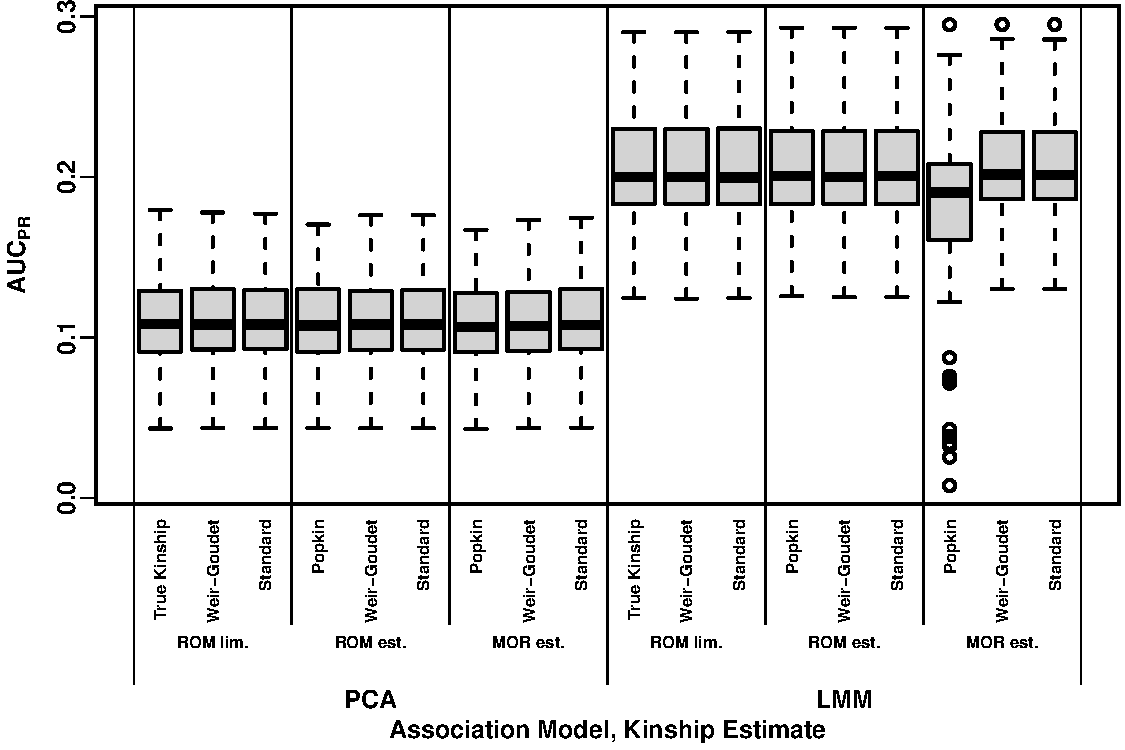
\includegraphics[width=\textwidth]{sim-admix-n1000-m100000-k3-f0.3-s0.5-mc100-h0.8-g20-fes/auc.pdf}
  \caption{
    {\bf Distributions of Area Under the Precision-Recall Curve ($\auc$) on the admixed family simulation.}
    Higher $\auc$ is better performance.
    Results for 100 replicates (each a random genotype matrix and trait vector).
    Approaches cluster primarily by association model (LMM or PCA), and do not depend much at all on the bias type.
  }
  \label{fig:auc_sim}
\end{figure}

% performance
We performed LMM and PCA association tests to determine how kinship biases affect association performance.
Surprisingly, we found that kinship bias type does not have a discernible effect on association performance, as summarized by $\auc$ (a robust proxy for power; \cref{fig:auc_sim}) and $\rmsd$ (measure null statistic calibration; \cref{fig:rmsd_sim}).
The largest differences in performance are explained by the association model used (LMM vs PCA), as expected due to our use of a family simulation, where PCA performs poorly.
Within association models, there are no clear differences between the performance of any of the kinship matrices, in fact many appear to have identical distributions (both statistics), the only clear exception being LMM popkin MOR, which has a few outlier replicates where performance was exceedingly poor.

\begin{figure}[bp!]
  \centering
  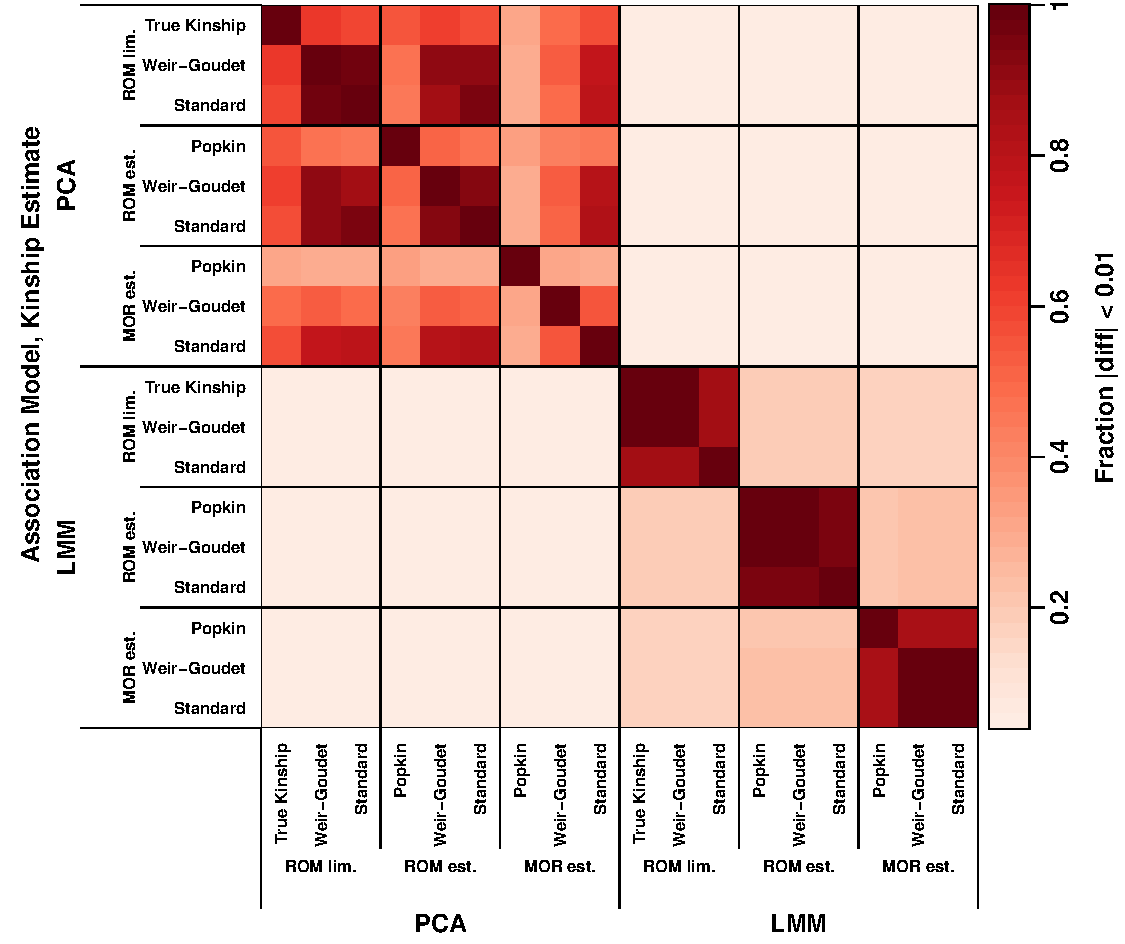
\includegraphics[width=\textwidth]{sim-admix-n1000-m100000-k3-f0.3-s0.5-mc100-h0.8-g20-fes/pvals_eq.pdf}
  \caption{
    {\bf Approximate agreement between p-values on the admixed family simulation.}
    The association p-value vector (one value per tested locus) produced by each combination of association model (LMM vs PCA) and kinship matrix (x and y axes) was used to compute proportions of loci with absolute differences under 0.01 (color).
    All 100 replicates were used.
    Methods of all bias types (matched for association model and locus weight type) have large proportions of nearly identical p-values.
    }
  \label{fig:pvals_eq_sim}
\end{figure}

% approximate agreement
To better characterize the nearly-identical performance distribution just observed, we next measured the agreement between individual association p-values.
We calculated the proportion of loci between two methods with p-values within 0.01 of each other, which is an approximate measure of agreement, and found a remarkably high agreement between estimators of diferent bias types after matching association model and locus-weight version or limit (\cref{fig:pvals_eq_sim}).
This is in contrast to the low amounts of agreement across PCA and LMM statistics, and even across LMM statistics with different locus-weight or between those and the ROM limits.
Minimum agreements tended to be higher across PCA methods, though here use of the true kinship or either popkin estimates resulted in more disagreements than between Standard and WG estimates or limits.
Overall, sets of matched kinship matrices except for different bias types result in nearly identical association statistics.

\subsection{Empirical analysis using 1000 Genomes}

% kinship
Now we repeat our analysis using the real genotypes of 1000 Genomes.
Kinship estimates are shown in \cref{fig:kinship_real} (note real data has no true kinship or estimator limits).
Popkin ROM estimates display an approximate nested block structure that arises from the tree relationships between subpopulations (\cref{fig:kinship_real}A; trees were explicitly fit to this data in previous work \citep{yao_limitations_2022}).
However, popkin MOR estimates do not follow the nested blocks tree structure, since kinship between African and non-African populations is higher than kinship within African populations (\cref{fig:kinship_real}B).
Standard estimates have values are closer to zero, and a different bias for each pair of individuals, resulting in higher relative kinship for African compared to non-African populations (\cref{fig:kinship_real}C-D).
Lastly, WG estimates are uniformly smaller than popkin's and attain large negative values (\cref{fig:kinship_real}E-F).

\begin{figure}[bp!]
  \centering
  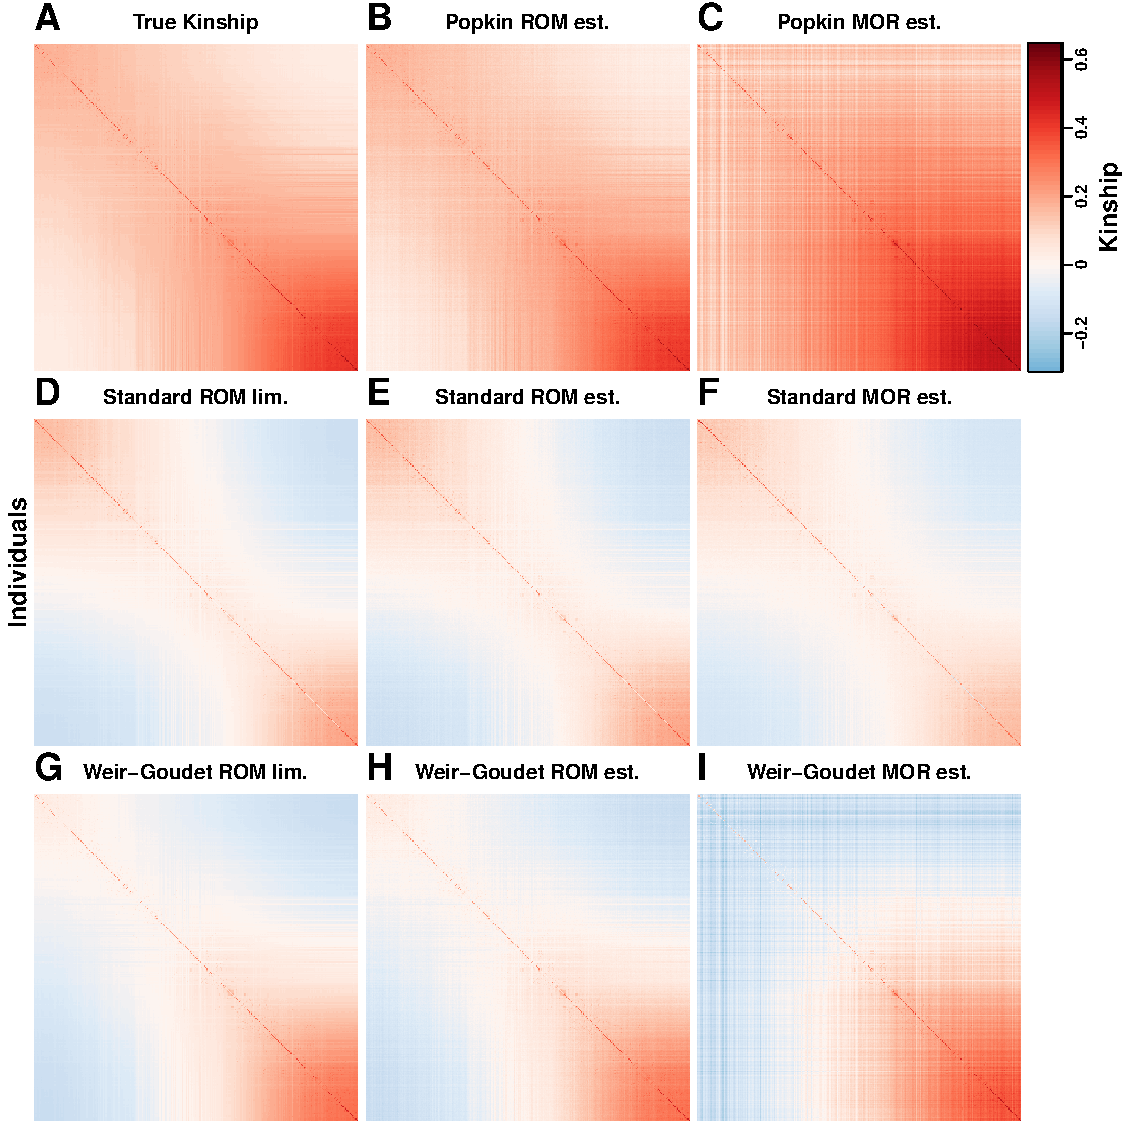
\includegraphics[height=0.8\textheight]{tgp-nygc-autosomes_ld_prune_1000kb_0.3_maf-0.01/kinship.pdf}
  \caption{
    {\bf Kinship estimates on 1000 Genomes.}
    Each panel represents a kinship matrix as a heatmap, as in \cref{fig:kinship_sim}.
    Superpopulation codes: AFR = African, EUR = European, SAS = South Asian, EAS = East Asian, AMR = Admixed Americans (Hispanics).
    Each estimator bias type (Popkin, Standard, and Weir-Goudet; rows) has two locus-weight versions (columns): ROM (ratio of means) and MOR (mean of ratios).
    In this visualization the upper range of all panels was capped to the 99 percentile of the diagonal (population inbreeding values) of the popkin MOR estimates.
  }
  \label{fig:kinship_real}
\end{figure}

% performance
Our association test conclusion are similar to our simulation study: $\auc$ and $\rmsd$ distributions are nearly identical for estimators of different bias types but same locus-weight version (ROM or MOR) and association model (\cref{fig:auc_real,fig:rmsd_real}).
However, unlike the simulation, here the MOR estimates greatly outperform ROM estimates (LMM only), on terms of both $\auc$ and $\rmsd$.
% agreement
P-values are again nearly identical at a large proportion of loci between approaches with matched association model and locus-weight version (MOR or ROM), regardless of bias type (\cref{fig:pvals_eq_real}).

\begin{figure}[bp!]
  \centering
  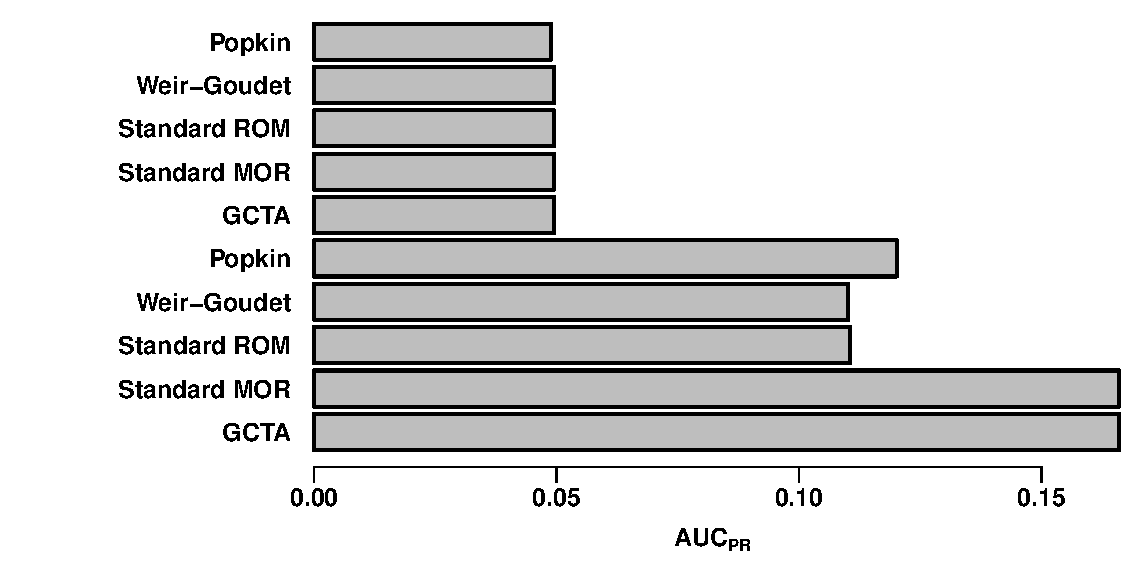
\includegraphics[width=\textwidth]{tgp-nygc-autosomes_ld_prune_1000kb_0.3_maf-0.01/auc.pdf}
  \caption{
    {\bf Distributions of Area Under the Precision-Recall Curve ($\auc$) on 1000 Genomes.}
    Higher $\auc$ is better performance.
    Results based on 100 simulated trait replicates (real genotype matrix is fixed).
    Approaches cluster primarily by association model (LMM or PCA) and locus-weight version (ROM or MOR), and do not depend much at all on the bias type.
  }
  \label{fig:auc_real}
\end{figure}

\subsection{Proof of association invariability to common kinship biases}

Our empirical observations suggested that replacing a kinship matrix with either the Standard- or WG-biased version does not alter association statistics (with exceptions we attribute to numerical computation artifacts); here prove a general version of these facts mathematically.
Our constructive proof shows that only a regression model with relatedness effects as covariates and an intercept is required, whose coefficients adapt to the bias, and no other coefficients change.
This is fortunate, as the intercept and relatedness coefficients are nuisance parameters that usually go unreported, while the focal genetic association coefficient and its p-value are unchanged by these biases.

The most general form we identified of the bias function, mapping a kinship matrix to its bias-transformed version, and for which association invariability holds, is
\begin{equation}
  \label{eq:kin-bias-general}
  \kinMatPrime
  =
  F \left( \kinMat \right)
  =
  \frac{1}{c}
  \mathbf{B} \kinMat \mathbf{B}^\intercal
  , \quad\quad
  \mathbf{B}
  =
  \mathbf{I} - \mathbf{1} \mathbf{b}^\intercal
  ,
\end{equation}
where $c$ is any positive scalar and $\mathbf{b}$ is any length-$n$ vector.

The Standard bias function $F = F^\text{std}$ of \cref{eq:kinship_std_lim} can be written as \cref{eq:kin-bias-general} with
$c = 1 - \bar{\varphi}^T$ and
$\mathbf{b} = \frac{1}{n} \mathbf{1}$, in which case $\mathbf{B}$ equals the centering matrix.
Further, the generalized standard kinship estimator studied in \citet{ochoa_estimating_2021} instead has $\mathbf{b}$ be the vector of individual weights used in the estimator, whose elements must sums to one, so $\mathbf{b}^\intercal \mathbf{1} = 1$.
In all these cases $\mathbf{B}$ and $\kinMatPrime$ are singular transformations, since $\mathbf{B} \mathbf{1} = \mathbf{0}$ and $\mathbf{B}^\intercal \mathbf{b} = \mathbf{0}$.

The WG bias function $F = F^\text{WG}$ of \cref{eq:wg_lim} can be written as \cref{eq:kin-bias-general} with
$c = 1 - \tilde{\varphi}^T$ and
\begin{align*}
  \mathbf{b}
  &=
    q \frac{ \left( \kinMat \right)^{-1} \mathbf{1} }{ \mathbf{1}^\intercal \left( \kinMat \right)^{-1} \mathbf{1} }
  , \\
  q
  &=
    1 \pm \sqrt{1 - (\mathbf{1}^\intercal \left( \kinMat \right)^{-1} \mathbf{1}) \tilde{\varphi}^T}
.
\end{align*}
The determinant of the quadratic solution $q$ is non-negative, since
$
\tilde{\varphi}^T \le 1 / (\mathbf{1}^\intercal \left( \kinMat \right)^{-1} \mathbf{1})
$
[TODO: prove it!], so both values of $b$ above are real.
This $\mathbf{b}$ does not sum to one ($\mathbf{b}^\intercal \mathbf{1} = q \ne 1$ [TODO: unless there's a degenerate case?]), so unlike the Standard bias case, here $\mathbf{B}$ is not evidently singular.
In fact, we prove that WG-biased kinship matrices are invertible if the original was invertible in \cref{sec:wg_posdef}.

\subsubsection{Proof for LMM case}

Consider a random effect $\mathbf{s}$ drawn using \kinMat, as given in \cref{eq:lmm_rand_eff}.
Using the affine transformation property of Multivariate Normal distributions (which despite its name also holds for singular linear transformations) and \cref{eq:kin-bias-general}, it follows that
$$
\mathbf{s}'
=
\mathbf{B} \mathbf{s}
\sim
\text{Normal} \left( \mathbf{0}, 2 (\sigma')^2 \kinMatPrime \right),
$$
where $(\sigma')^2 = c \sigma^2$.
(This $\mathbf{s}'$ has a degenerate distribution for Standard bias, since $\kinMatPrime$ is singular, but this is not problematic as long as $\mathbf{s}' + \boldsymbol{\epsilon}$ is non-degenerate, whose total covariance $(\sigma')^2 \kinMatPrime + \sigma^2_\epsilon \mathbf{I}$ is invertible as long as $\sigma^2_\epsilon \ne 0$.)
The key property that $\mathbf{B}$ must satisfy for association invariability is that
$
\mathbf{B} \mathbf{s}
=
\mathbf{s} - \mathbf{1} \eta
,
$
where $\eta = \mathbf{b}^\intercal \mathbf{s}$ is a scalar, so
$$
\mathbf{s}' = \mathbf{s} - \mathbf{1} \eta
$$
are equal in distribution.
Therefore, after matching the variance coefficients $\sigma^2$ and $(\sigma')^2$ as above, the random effect $\mathbf{s}'$ of the biased kinship matrix differs from the random effect $\mathbf{s}$ of the original kinship only by $\mathbf{1} \eta$, a difference compensated for by adjusting the intercept coefficient in \cref{eq:lmm_gwas}: $\alpha' = \alpha + \eta$.
No other regression coefficients, or the total residuals, change when \kinMat is replaced with $\kinMatPrime$, including the association coefficient $\beta_i$ that is the focus of the test.

The LMM association p-value does not change in several common tests, including the F-test, since it only depends on the residuals and these do not change, as well as the likelihood ratio test, because although the covariance matrices do change, their determinants cancel out in the ratio.
[TODO: What about Score, Wald tests?  I think there can be changes in one of those cases!]
The argument holds whether the model is fit with maximum likelihood (ML) or restricted maximum likelihood (REML) \citep{kang_efficient_2008}, since the difference only affects how $\sigma^2$ is estimated, and in both cases the adjusted estimate, which is given by the original $\sigma^2$ multiplied by $c$, results in an identical likelihood so no other estimates are affected.

\subsubsection{Proof for PCA case}

We present a proof for the PCA case that relies on an approximation that holds well in practice.
Based on the PCA model of \cref{eq:pca_gwas,eq:kin_evd}, let $\mathbf{U}_d$ be the top eigenvectors of \kinMat, and $\mathbf{U}_d'$ those of $\kinMatPrime$.
They key approximation is that
$$
\mathbf{U}_d' \approx \mathbf{B} \mathbf{U}_d,
$$
which is not strictly equal (since $\mathbf{B} \mathbf{U}$ is not generally orthogonal, as eigenvectors must be), but we have found it to be a good approximation in practice.
In this case the eigenvector coefficients need not change, $\boldsymbol{\gamma}_d' = \boldsymbol{\gamma}_d$, since the difference in scale of the kinship matrices ($c$ in \cref{eq:kin-bias-general}) is absorbed by the eigenvalues, which are not used in the association model.
As before, note that
$$
\mathbf{U}_d' \boldsymbol{\gamma}_d'
=
\mathbf{B} \mathbf{U}_d \boldsymbol{\gamma}_d
=
\mathbf{U}_d \boldsymbol{\gamma}_d - \mathbf{1} \eta,
$$
where
$\eta = \mathbf{b}^\intercal \mathbf{U}_d \boldsymbol{\gamma}_d$
is a scalar.
Therefore, the relatedness effects again differ only by $\mathbf{1} \eta$, which is compensated for by adjusting the intercept accordingly, so the association coefficient $\beta_i$ and the residuals are the same in both cases.
The observations from LMMs, for how p-values change depending on the type of test used, also hold for PCA.

\subsection{Proof of association invariability to change in ancestral population}

The kinship matrices we have used so far have values that depend on the choice of ancestral population $T$.
Here we consider the effect on association of changing ancestral population, and prove that it is compensated for by the relatedness and intercept coefficients, just as it was for common kinship biases.

Suppose we had started with a kinship matrix \kinMat[S] in terms of ancestral population $S$, and $T$ is a population ancestral to $S$.
If the inbreeding coefficient of $S$ when $T$ is the reference ancestral population is $\f{T}{S}$, then the kinship matrix \kinMat in terms of $T$ is given by \citep{ochoa_estimating_2021}
$$
\left( \mathbf{J} - \kinMat \right)
=
\left( \mathbf{J} - \kinMat[S] \right) \left( 1 - \f{T}{S} \right)
.
$$
Solving for \kinMat and simplifying results in
$$
\kinMat
=
\left( 1 - \f{T}{S} \right) \kinMat[S] + \f{T}{S} \mathbf{J}
.
$$
Notice that this resembles the WG bias function but in reverse: whereas WG bias reduces and rescales all kinship values by $\tilde{\varphi}^T$, changing to a more ancestral population rescales and increases all kinship values by \f{T}{S}.
Indeed, excluding the degenerate case $\f{T}{S} = 1$, this transformation can be written as \cref{eq:kin-bias-general} with
$c = \left( 1 - \f{T}{S} \right)^{-1}$ and
\begin{align*}
  \mathbf{b}
  &=
    q \frac{ \left( \kinMat[S] \right)^{-1} \mathbf{1} }{ \mathbf{1}^\intercal \left( \kinMat[S] \right)^{-1} \mathbf{1} }
  , \\
  q
  &=
    1 \pm \sqrt{1 + (\mathbf{1}^\intercal \left( \kinMat[S] \right)^{-1} \mathbf{1}) \f{T}{S} \left( 1 - \f{T}{S} \right)^{-1} }
.
\end{align*}
The determinant of $q$ is strictly positive, since $\mathbf{1}^\intercal \left( \kinMat[S] \right)^{-1} \mathbf{1} > 0$ (since \kinMat[S] is positive definite, its inverse is too) and $0 \le \f{T}{S} < 1$.
Thus, the results of the previous section also apply to this transformation: ancestor change is also compensated for by the relatedness and intercept coefficients, which are the only coefficients that depend on the ancestor population, so the association statistics are invariant to this transformation.

\section{Discussion}

% association robust to bias type (empirical and theory / summary)
Previous research showed that commonly used kinship estimators are biased, and that these biases can be large (\citet{ochoa_estimating_2021}; \cref{fig:kinship_sim}).
We initiated the present work under the hypothesis that these kinship biases would affect association testing, but surprisingly find that association is unaffected by these kinship biases.
We then prove theoretically that it is the intercept and relatedness (random effect or PCs) coefficients that compensate for the bias, and result in identical genetic effect coefficients and significance statistics.

% ancestor population
One previously uncomfortable fact was that kinship estimates depend on the choice of ancestral population, which conditions the distributions of allele frequencies and genotypes, but the effect of this choice of association testing was not only unknown but completely disregarded.
A corollary of our theoretical results is that changes of ancestral population, which behave algebraically like the reverse of the WG kinship bias, are also compensated for by the relatedness and intercept coefficients, so association testing is also invariant to the choice of ancestral population.
Thus, although a choice of ancestral population is always being made when estimating kinship, this choice is fortunately inconsequential to association testing, as it ought to be since the relatedness structure overall is being conditioned upon in these tests.

% popkin is less numerically stable
Given that kinship bias type is not important for association studies, we are free to choose a kinship estimator based on other properties.
The biased standard kinship matrix may be more desirable than the popkin estimator based on the numerical stability we observed in our simulations.
In particular, while theory shows that the solutions should be the same for all estimators of the same type, we find that popkin's statistics disagree more often from the standard and WG estimators, namely LMM association with popkin MOR (admixed family simulation, \cref{fig:auc_sim}, \cref{fig:rmsd_sim}) and popkin ROM (1000 Genomes, \cref{fig:rmsd_real}).
The standard kinship matrix is orthogonal to the intercept, because of the centering operation applied to obtain it in our theoretical results, whereas the popkin and true kinship matrices are not orthogonal to the intercept.
Thus, PCA regression with the eigenvectors of the standard kinship matrix is more numerically stable (because more covariates are linearly independent) than the popkin counterpart.
We believe that the observed popkin disagreemnts in LMMs are due to poor convergence of that algorithm in those cases.

% MOR weirdness
We also found that all MOR estimators perform better in the LMM association (and overall) compared to the ROM versions in the 1000 Genomes evaluation.
Perhaps this is expected because out trait simulation follows the ``fixed effect sizes'' model, in which rare variants have larger coefficients, and the MOR estimators also weigh rare variants more highly in estimating kinship coefficients.
This effect was not observed in the admixed family simulation, where MOR and ROM versions gave similar kinship estimates and performed similarly, compared to the real data evaluation, where kinship estimates were also strikingly different.
However, only the popkin ROM estimator is unbiased (\cref{fig:kinship_sim}B, \cref{fig:popkin-rom-mor}), so it is unclear why the biased popkin MOR estimator performs better in this setting.
One potential explanation is that our kinship model assumes that all variants were preexisting in the MRCA population, whereas rare variants in human data are known to be very recent mutations, and thus their effective kinship matrix is different than that of ancestral variants.
Therefore, despite its biases, it is possible that the popkin MOR estimator is more accurately capturing the kinship matrix of these rare variants and thus modeling them better in association tests, particularly in LMMs where the effect is most pronounced.

% implications for other estimators
Our conclusions extend to variants of the standard kinship estimator that weigh loci according to linkage disequilibrium \citep{speed_reevaluation_2017, wang_efficient_2017}, which have the same bias form since this bias is present in each individual locus \citep{ochoa_estimating_2021}.
As shown in our proof, the more general form of the standard kinship estimator that weighs individuals to estimate ancestral allele frequencies \pith is also subject to the same conclusions.
Such weighted \pith estimates include the best unbiased linear estimator \citep{astle_population_2009, thornton_roadtrips:_2010}.

% conclusion / take away
In this study, we show empirically and theoretically that association tests are invariant to the use of common kinship estimators that are biased as well as a more recent unbiased estimator.
% future work / implication beyond this work
The theoretical underpinnings of our proof show that the same is expected of any generalized linear model with the same setup, namely intercept and population structure with coefficients that are nuisance variables, which includes case/control models as well as the quantitative trait model we explicitly studied here.
However, heritability estimation requires unbiased estimates of the random effect coefficient ($\sigma^2$), so our results prove that it will be biased when the standard kinship estimator is used, as it is using GCTA \citep{yang_gcta:_2011, yang_advantages_2014}.
Nevertheless, heritability estimation is a complex problem and its full study is beyond the scope of this work.
Overall, we have described an unexpected robustness of association studies, and our theoretical understanding of this result may help guide future improvements for association and other related models.



\section*{Declaration of interests}
The authors declare no competing interests.

\section*{Acknowledgments}
This work was funded in part by the Duke University School of Medicine Whitehead Scholars Program, a gift from the Whitehead Charitable Foundation.
The 1000 Genomes data were generated at the New York Genome Center with funds provided by NHGRI Grant 3UM1HG008901-03S1.

\section*{Web resources}
plink2, \url{https://www.cog-genomics.org/plink/2.0/}\\
GCTA, \url{https://yanglab.westlake.edu.cn/software/gcta/}\\
bnpsd, \url{https://cran.r-project.org/package=bnpsd}\\
simfam, \url{https://cran.r-project.org/package=simfam}\\
simtrait, \url{https://cran.r-project.org/package=simtrait}\\
popkin, \url{https://cran.r-project.org/package=popkin}\\
popkinsuppl, \url{https://github.com/OchoaLab/popkinsuppl}

\section*{Data and code availability}
The data and code generated during this study are available on GitHub at \url{https://github.com/OchoaLab/bias-assoc-paper}.
The high-coverage version of the 1000 Genomes Project was downloaded from \url{ftp://ftp.1000genomes.ebi.ac.uk/vol1/ftp/data_collections/1000G_2504_high_coverage/working/20190425_NYGC_GATK/}.


\printbibliography


\begin{appendices}
  \appendix

  \appendixpage
  
  \section{Justification for popkin generalizations}

  \label{sec:popkin_w_justif}

  The popkin estimator in \cref{eq:popkin} has been generalized in this work to include locus weights $w_i$.
  The original formulation had $w_i=1$ for all loci $i$ \citep{ochoa_estimating_2021}.
  Recalling from that original work that
  $$
  \E \left[ (\xij-1)(\xij[k]-1) - 1 \middle| T \right]
  =
  4 \pit \left( 1 - \pit \right) \left( \kt - 1 \right),
  $$
  then for fixed $w_i$ we get
  \begin{align*}
    \E \left[ \Ajk \middle| T \right]
    &=
      v_m^T \left( \kt - 1 \right)
      , \\
    v_m^T
    &=
      \frac{4}{m} \sum_{i=1}^m w_i \pit \left( 1 - \pit \right)
      .
  \end{align*}
  Therefore, as before all the unknowns \pit and now also the (known) weights $w_i$ collapse into a single parameter $v_m^T$, which is estimated under the assumption that the minimum kinship is zero, giving $\AMinHat = -v_m^T$, so that
  $$
  \ktHatNamed{popkin-ROM}
  =
  1 - \frac{\Ajk}{\AMinHat}
  \toas
  \kt
  $$
  as desired.

  The MOR case of $w_i = \left( \pith \left( 1 - \pith \right) \right)^{-1}$ does not fit the previous case because this $w_i$ is a random variable (it is a function of the genotypes).
  The term of interest $w_i ( (\xij-1)(\xij[k]-1) - 1 )$ is a ratio of random variables whose expectation does not have a closed form.
  In this case, we rely on the first-order approximation to this expectation, namely
  \begin{align*}
    \E \left[ \frac{ (\xij-1)(\xij[k]-1) - 1 }{ \pith \left( 1 - \pith \right) } \middle| T \right]
    &\approx
      \frac{ \E \left[ (\xij-1)(\xij[k]-1) - 1 \middle| T \right] }{ \E \left[ \pith \left( 1 - \pith \right) \middle| T \right] }
    \\
    &=
      \frac{ 4 \pit \left( 1 - \pit \right) \left( \kt - 1 \right) }{ \pit \left( 1 - \pit \right) \left( 1 - \bar{\varphi}^T \right) }
    \\
    &=
      \frac{ 4 \left( \kt - 1 \right) }{ 1 - \bar{\varphi}^T }
  ,
  \end{align*}
  where the expectation of $\pith \left( 1 - \pith \right)$ was calculated previously \citep{ochoa_estimating_2021}.
  In this case the expectation of \Ajk, summing across loci, is also approximated by
  $$
  \E \left[ \Ajk \middle| T \right]
  \approx
  \frac{ 4 \left( \kt - 1 \right) }{ 1 - \bar{\varphi}^T }
  .
  $$
  The same strategy as before applies to estimate the unknown factor $4 / \left( 1- \bar{\varphi}^T \right)$, namely that if the minimum kinship is zero then $\AMinHat \approx - 4 / \left( 1- \bar{\varphi}^T \right)$, resulting in
  $$
  \ktHatNamed{popkin-MOR}
  =
  1 - \frac{\Ajk}{\AMinHat}
  \approx
  \kt
  .
  $$

  \section{Connection between popkin and standard kinship estimator}

  \label{sec:conn_popkin_std}  

  Since the conection we discovered holds when data is complete but not under missingness, to determine necessary conditions, here we introduce more complete forms of the estimators that handle missingness.
  The generalized popkin estimator (including both ROM and MOR special cases) is
  \begin{equation*}
    %\label{eq:popkin_miss}
    \begin{split}
      A_{ijk}
      &=
        I_{ij} I_{ik} ( (\xij-1)(\xij[k]-1) - 1 )
      , \\
      \Ajk
      &=
        \frac{1}{m_{jk}} \sum_{i=1}^m w_i A_{ijk}
        , \\
      m_{jk}
      &=
        \sum_{i=1}^m I_{ij} I_{ik}
        ,
    \end{split}
  \end{equation*}
  where $I_{ij} = 1$ if \xij is not missing, 0 otherwise (this way missing \xij can be treated as having any finite value and not contribute to the estimator).
  Note that only loci where both genotypes ($\xij$ and $\xij[k]$) are non-missing are included in the above average, and $m_{jk}$ counts the total number of such loci.
  The ancestral allele frequency estimator with missingness is
  \begin{align*}
    \pith
    &=
      \frac{1}{2 n_i} \sum_{j=1}^n I_{ij} \xij
      , \\
    n_i
    &=
      \sum_{j=1}^n I_{ij}
      ,
  \end{align*}
  which averages over individuals rather than loci, so its denominator is the number of non-missing individuals at this locus.
  Let us compute some averages of the generalized popkin estimator.
  Since the result we want holds at every locus separately, let us formulate the averages of interest at locus $i$ only:
  \begin{align*}
    \bar{A}_{ij}
    &=
      \frac{1}{n} \sum_{k=1}^n A_{ijk}
      =
      I_{ij} \frac{n_i}{n} \left( ( \xij - 1 ) \left( 2 \pith - 1 \right) - 1 \right)
      , \\
    \bar{A}_i
    &=
      \frac{1}{n} \sum_{k=1}^n \bar{A}_{ij}
      =
      - \left( \frac{n_i}{n} \right)^2 4 \pith \left( 1 - \pith \right)
      .
  \end{align*}
  Therefore, the combination of interest is:
  \begin{align*}
    A_{ijk} + \bar{A}_i - \bar{A}_{ij}  - \bar{A}_{ik}
    % &=
    %   I_{ij} I_{ik} ( (\xij-1)(\xij[k]-1) - 1 )
    %   - \left( \frac{n_i}{n} \right)^2 4 \pith ( 1 - \pith )
    %   - I_{ij} \frac{n_i}{n} ( ( \xij - 1 )( 2 \pith - 1 ) - 1 )
    %   - I_{ik} \frac{n_i}{n} ( ( \xij[k] - 1 )( 2 \pith - 1 ) - 1 )
    % \\
    &=
      I_{ij} I_{ik} \left( \xij - 2 \pith \right) \left( \xij[k] - 2 \pith \right)
    \\
      &+ \frac{n_i}{n} \left( I_{ij} - \frac{n_i}{n} \right) 4 \pith
        + \left( \left( \frac{n_i}{n} \right)^2 -  I_{ij} I_{ik} \right) 4 \left( \pith \right)^2
    \\
      &+ I_{ij} \left( I_{ik} - \frac{n_i}{n} \right) \xij \left( 2 \pith - 1 \right)
      + I_{ik} \left( I_{ij} - \frac{n_i}{n} \right) \xij[k] \left( 2 \pith - 1 \right)
      .
  \end{align*}
  To arrive at the desired result of $I_{ij} I_{ik} \left( \xij - 2 \pith \right) \left( \xij[k] - 2 \pith \right)$, which is the first term above, it is necessary for the rest of the terms to vanish for arbitrary values of \pith, \xij, and \xij[k].
  Since $n_i > 0$ (there is at least one non-missing individual at every locus), the term $\frac{n_i}{n} ( I_{ij} - \frac{n_i}{n} ) 4 \pith$ vanishes if and only if $I_{ij} = \frac{n_i}{n}$, and since $I_{jk}=0$ does not solve this equation (because $n_i > 0$) the only other case is $I_{jk}=1$, which requires $n_i=n$, so no individuals can have missing data at this locus.
  Thus,
  $$
  A_{ijk} + \bar{A}_i - \bar{A}_{ij}  - \bar{A}_{ik}
  =
  I_{ij} I_{ik} \left( \xij - 2 \pith \right) \left( \xij[k] - 2 \pith \right)
  $$
  if and only if there is no missing data at locus $i$.
  The other desired result of
  $$
  \bar{A}_i
  =
  - 4 \pith \left( 1 - \pith \right)
  $$
  also requires $n_i = n$.

  Assuming now no missingness, transforming the popkin estimates as desired gives
  \begin{align*}
    \frac{
    \ktHatNamed{popkin}
    + \bar{ \hat{ \varphi } }^{T,\text{popkin}}
    - \bar{ \hat{ \varphi } }_j^{T,\text{popkin}}
    - \bar{ \hat{ \varphi } }_k^{T,\text{popkin}}
    }{
    1 - \bar{ \hat{ \varphi } }^{T,\text{popkin}}
    }
    % &=
    %   \frac{
    %   ( 1 - \frac{\Ajk}{\AMinHat} )
    %   + ( 1 - \frac{\bar{A}}{\AMinHat} )
    %   - ( 1 - \frac{\bar{A}_j}{\AMinHat} )
    %   - ( 1 - \frac{\bar{A}_k}{\AMinHat} )
    %   }{
    %   \frac{\bar{A}}{\AMinHat}
    %   }
    % \\
    &=
      \frac{
      \Ajk
      + \bar{A}
      - \bar{A}_j
      - \bar{A}_k
      }{
      - \bar{A}
      }
    \\
    &=
      \frac{
      \sum_{i=1}^m w_i ( A_{ijk} + \bar{A}_i - \bar{A}_{ij} - \bar{A}_{ik} )
      }{
      - \sum_{i=1}^m w_i \bar{A}_i
      }
    \\
    &=
      \frac{
      \sum_{i=1}^m w_i \left( \xij - 2 \pith \right) \left( \xij[k] - 2 \pith \right)
      }{
      \sum_{i=1}^m w_i 4 \pith \left( 1 - \pith \right)
      }
      .
  \end{align*}
  Therefore, if popkin-ROM is input ($w_i=1$), this transformation yields std-ROM.
  On the other hand, if popkin-MOR is used ($w_i^{-1} = \pith \left( 1 - \pith \right)$), the transformation yields std-MOR.
  
  \section{Proof that WG limits are positive definite}

  \label{sec:wg_posdef}

  Starting from a positive-definite kinship matrix \kinMat, we prove that WG-bias transformed matrix $\kinMatPrime = F^\text{WG}( \kinMat )$ is also positive definite (and therefore invertible), except in one degenerate case.
  Recall from \cref{eq:wg_lim} that
  $
  \kinMatPrime
  =
  \frac{1}{1-\tilde{\varphi}^T} \left( \kinMat - \tilde{\varphi}^T \boldsymbol{J} \right)
  .
  $
  We shall not consider $\kinMat = \mathbf{J}$ as a valid kinship matrix, which therefore ensures that $\tilde{\varphi}^T < 1$ as there is at least one kinship value with $\kt < 1$.
  Now consider two linear subspaces of $\mathbb{R}^n$, $S_1$ spanned by $\mathbf{1}$ and $S_2$ its complement (orthogonal to $\mathbf{1}$), and prove that $\kinMatPrime$ is positive definite in both subspaces, therefore it is positive-definite in the direct sum of the subspaces, which equals the entire space: $\mathbb{R}^n = S_1 \oplus S_2$.
  (This follows since vectors $\mathbf{v}$ for which $\kinMatPrime$ is not positive definite, if they exist, span a linear subspace, but its intersection to $S_1$, $S_2$, and therefore $S_1 \oplus S_2$, is trivial \citep{hefferon_linear_2020}.)
  In both subspaces we will prove that $\mathbf{v} \in S_i$ and $\mathbf{v} \ne \mathbf{0}$ implies $\mathbf{v}^\intercal \kinMatPrime \mathbf{v} > 0$ which proves that $\kinMatPrime$ is positive definite in that subspace.

  We begin by considering $\mathbf{v} \in S_2$, which satisfy $\mathbf{1}^\intercal \mathbf{v} = \mathbf{0}$, and by hypothesis $\mathbf{v} \ne \mathbf{0}$.
  Therefore $\mathbf{v}^\intercal \mathbf{J} \mathbf{v} = 0$ in this subspace, which results in
  $$
  \mathbf{v}^\intercal \kinMatPrime \mathbf{v}
  =
  \frac{1}{1-\tilde{\varphi}^T} \mathbf{v}^\intercal \kinMat \mathbf{v}
  >
  0
  ,
  $$
  where the final inequality follows since the original kinship matrix is positive definite and $1-\tilde{\varphi}^T > 0$.

  Lastly, we consider $\mathbf{v} \in S_1$, which are necessarily of the form $\mathbf{v} = v \mathbf{1}$, and by hypothesis $v \ne 0$.
  Therefore
  $$
  \mathbf{v}^\intercal \kinMatPrime \mathbf{v}
  =
  \frac{ v^2 }{1-\tilde{\varphi}^T}(\boldsymbol{1^\intercal \kinMat 1} - \tilde{\varphi}^T n^2)
  =
  \frac{ v^2 n^2 }{1-\tilde{\varphi}^T} \left( \bar{\varphi}^T - \tilde{\varphi}^T \right)
  ,
  $$
  where $\bar{\varphi}^T$ is the overall mean kinship value, while $\tilde{\varphi}^T$ is the mean of the off-diagonal kinship values only (\cref{eq:wg_tilde}).
  Note that $v^2, n^2, 1 - \tilde{\varphi}^T > 0$, so the desired result follows if $\tilde{\varphi}^T < \bar{\varphi}^T$, which is proven in \cref{sec:mean_kinship_ineqs}.
  In general it is true that $\tilde{\varphi}^T \le \bar{\varphi}^T$, and $\tilde{\varphi}^T = \bar{\varphi}^T$ occurs if and only if the kinship matrix has the degenerate form $\kinMat = \bar{\varphi}^T \mathbf{J}$, which is a singular matrix not expected in practice (in this case $\kinMatPrime$ is a matrix full of zeroes).

  \section{Mean kinship inequalities}

  \label{sec:mean_kinship_ineqs}

  Denote the mean of the diagonal kinship terms as $\bar{\delta}^T = \frac{1}{n} \sum_{j=1}^n \kt[j]$.
  Here we prove that
  $$
  0 \le \tilde{\varphi}^T \le \bar{\varphi}^T \le \bar{\delta}^T \le 1,
  $$
  with each of $\tilde{\varphi}^T = \bar{\varphi}^T$ and $\bar{\varphi}^T = \bar{\delta}^T$ if and only if all kinship values are equal.

  The inequalities $0 \le \bar{\varphi}^T \le \bar{\delta}^T \le 1$ follow directly from previous work, applied to a kinship matrix rather than a coancestry matrix as done originally, as the proof required solely a covariance matrix with values between 0 and 1 \citep{ochoa_estimating_2021}.
  Recall that $\tilde{\varphi}^T$ is defined in \cref{eq:wg_tilde}.
  The lower bound $0 \le \tilde{\varphi}^T$ follows since every kinship value is non-negative.
  Note that $\bar{\varphi}^T$ and $\tilde{\varphi}^T$ are related by
  \begin{equation}
    \label{eq:kinship_mean_tilde}
    \bar{\varphi}^T
    =
    \frac{ \tilde{\varphi}^T (n-1) + \bar{\delta}^T }{n}.
  \end{equation}
  Applying $\bar{\varphi}^T \le \bar{\delta}^T$ to \cref{eq:kinship_mean_tilde} and simplifying yields $\tilde{\varphi}^T \le \bar{\delta}^T$.
  Lastly, since $\bar{\varphi}^T - \tilde{\varphi}^T = \left( \bar{\delta}^T - \tilde{\varphi}^T \right) / n$ (from rearranging \cref{eq:kinship_mean_tilde}), it also follows that $\tilde{\varphi}^T \le \bar{\varphi}^T$, as desired.
  Furthermore, $\tilde{\varphi}^T = \bar{\varphi}^T$ holds if and only if all $\kt = \bar{\delta}^T$, since that is necessary and sufficient for $\bar{\varphi}^T = \bar{\delta}^T$.

\end{appendices}



%%%%%%%%%%%%%%%%%%%%%%%%%%%%%%%%% 
%%% SUPPLEMENTARY INFORMATION %%%
%%%%%%%%%%%%%%%%%%%%%%%%%%%%%%%%%

\clearpage

\beginsupplement

\section*{Supplemental figures}

\begin{figure}[hp!]
  \centering
  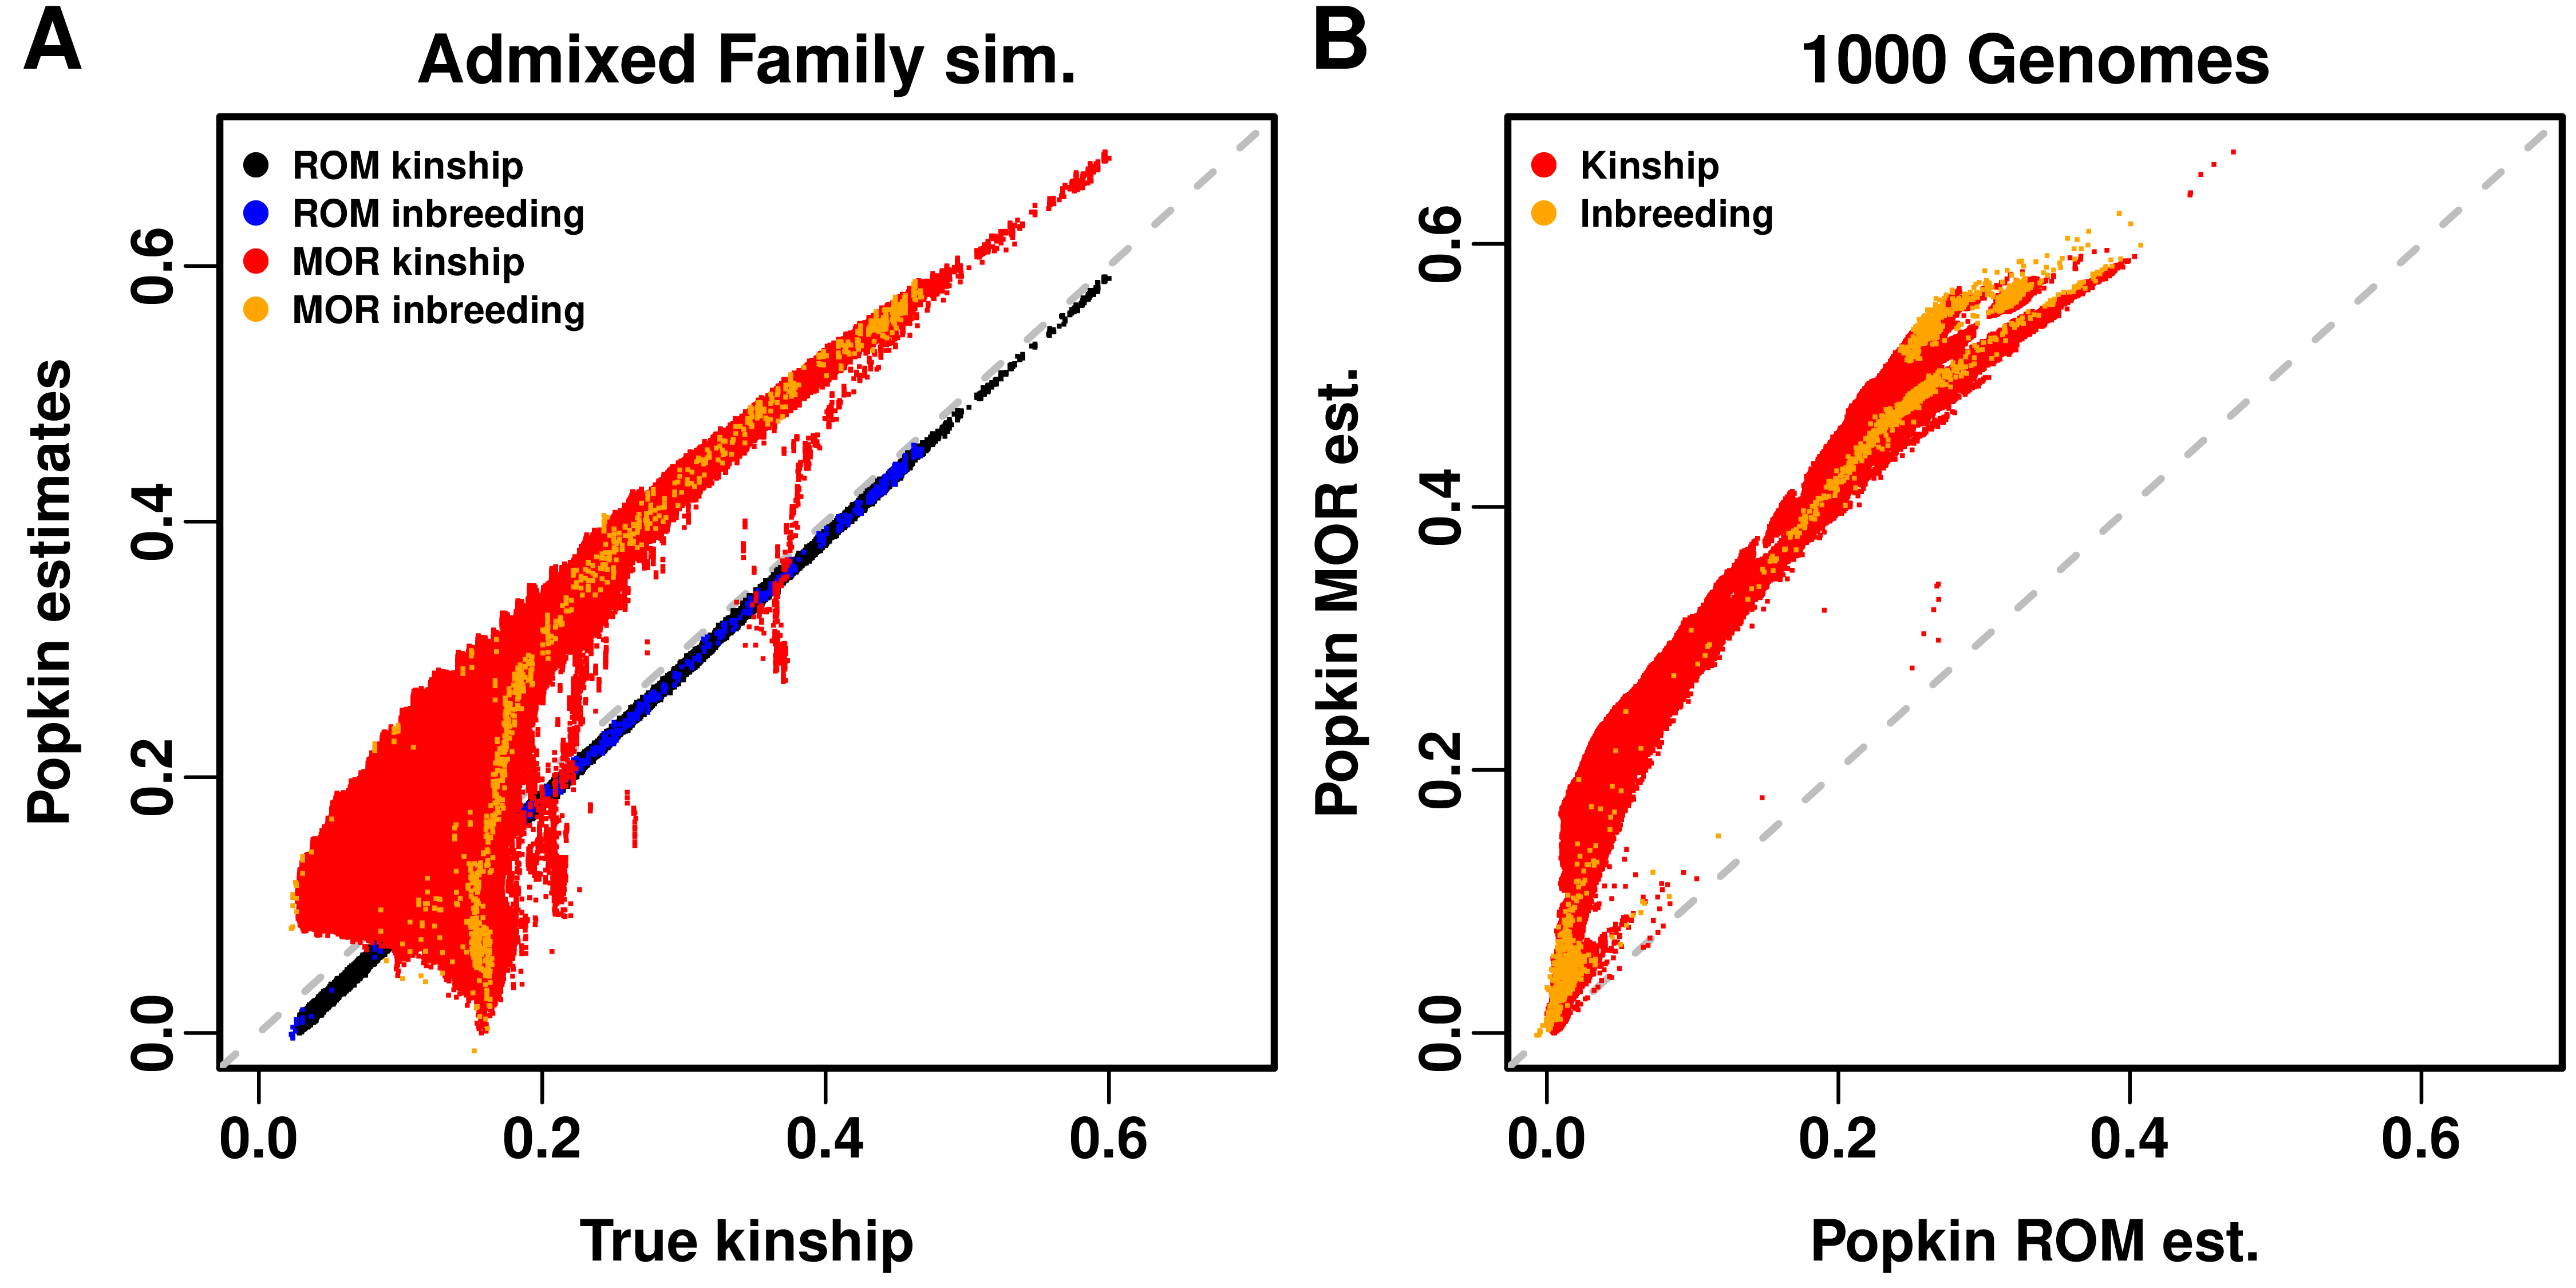
\includegraphics[width=\textwidth]{popkin-mor-rom-bias.png}
  \caption{
    {\bf Comparison of popkin ROM and MOR estimates.}
    Kinship (off-diagonal of matrix) and inbreeding (transformed diagonal) are plotted in different colors, which shows that their biases (if any) overlap.
    \textbf{A.}
    In admixed family simulation, both estimates are compared against true kinship.
    Popkin ROM has a negligible bias, due to the minimum true kinship of the simulation being slightly larger than zero.
    Popkin MOR has considerable biases, tending to be upward though not always.
    \textbf{B.}
    In 1000 Genomes, since true kinship is unknown, popkin ROM takes its place.
    Popkin MOR biases take on a similar shape as panel A.
    }
  \label{fig:popkin-rom-mor}
\end{figure}

\begin{figure}[hp!]
  \centering
  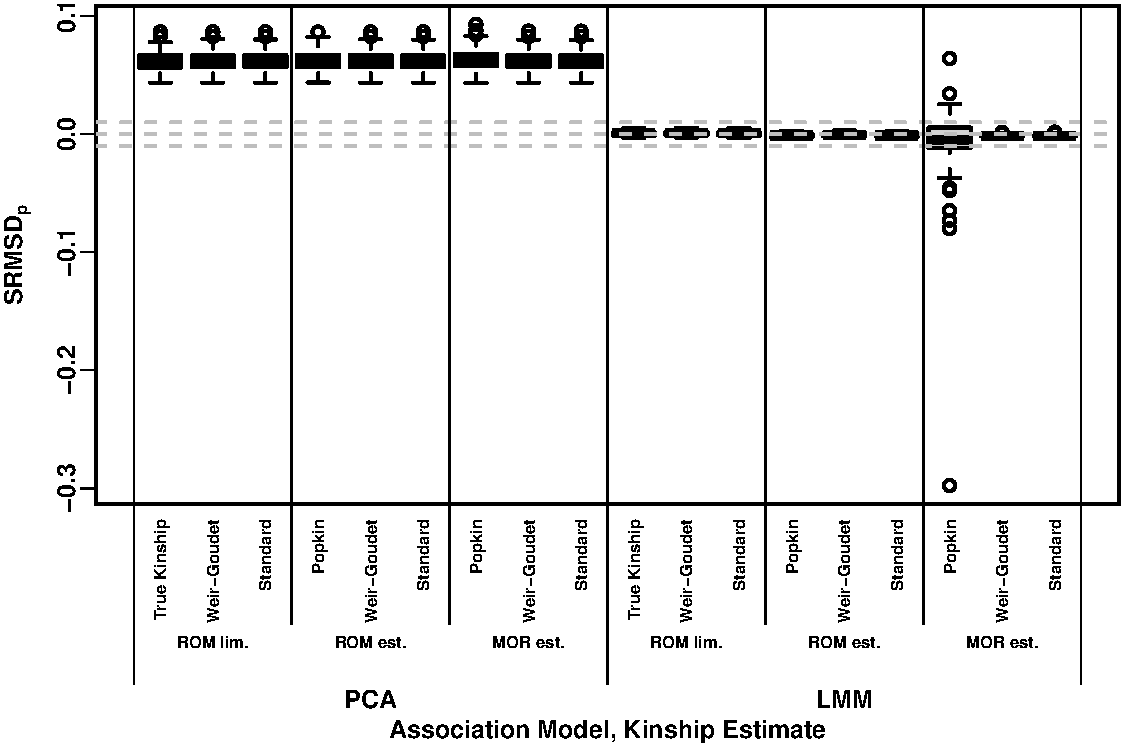
\includegraphics[width=\textwidth]{sim-admix-n1000-m100000-k3-f0.3-s0.5-mc100-h0.8-g20-fes/rmsd.pdf}
  \caption{
    {\bf Signed Root Mean Square Deviation of null p-values ($\rmsd$) on the admixed family simulation.}
    Same methods and simulation as \cref{fig:auc_sim}, see that for more information.
    $|\rmsd| < 0.01$ (area between gray dashed lines) is considered calibrated.
    All PCA runs are miscalibrated by similar amounts, whereas most LMM runs are calibrated with few exceptions.
    }
  \label{fig:rmsd_sim}
\end{figure}

\begin{figure}[hp!]
  \centering
  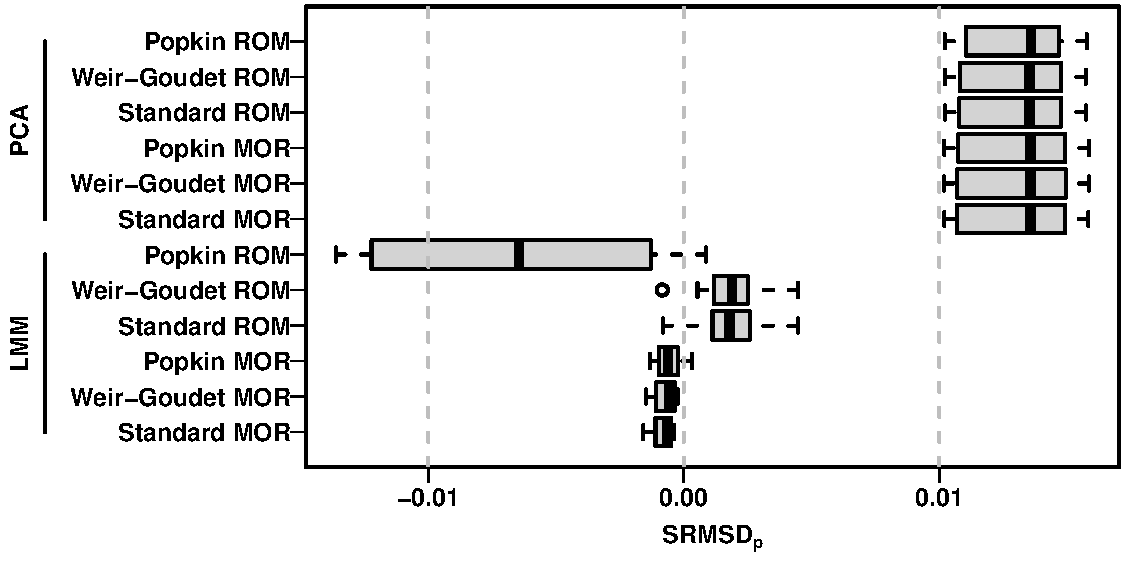
\includegraphics[width=\textwidth]{tgp-nygc-autosomes_ld_prune_1000kb_0.3_maf-0.01/rmsd.pdf}
  \caption{
    {\bf Signed Root Mean Square Deviation of null p-values ($\rmsd$) on 1000 Genomes.}
    Same methods and simulation as \cref{fig:auc_real}, and y-axis statistic and conclusions of \cref{fig:rmsd_sim}, see those for more information.
  }
  \label{fig:rmsd_real}
\end{figure}

\begin{figure}[bp!]
  \centering
  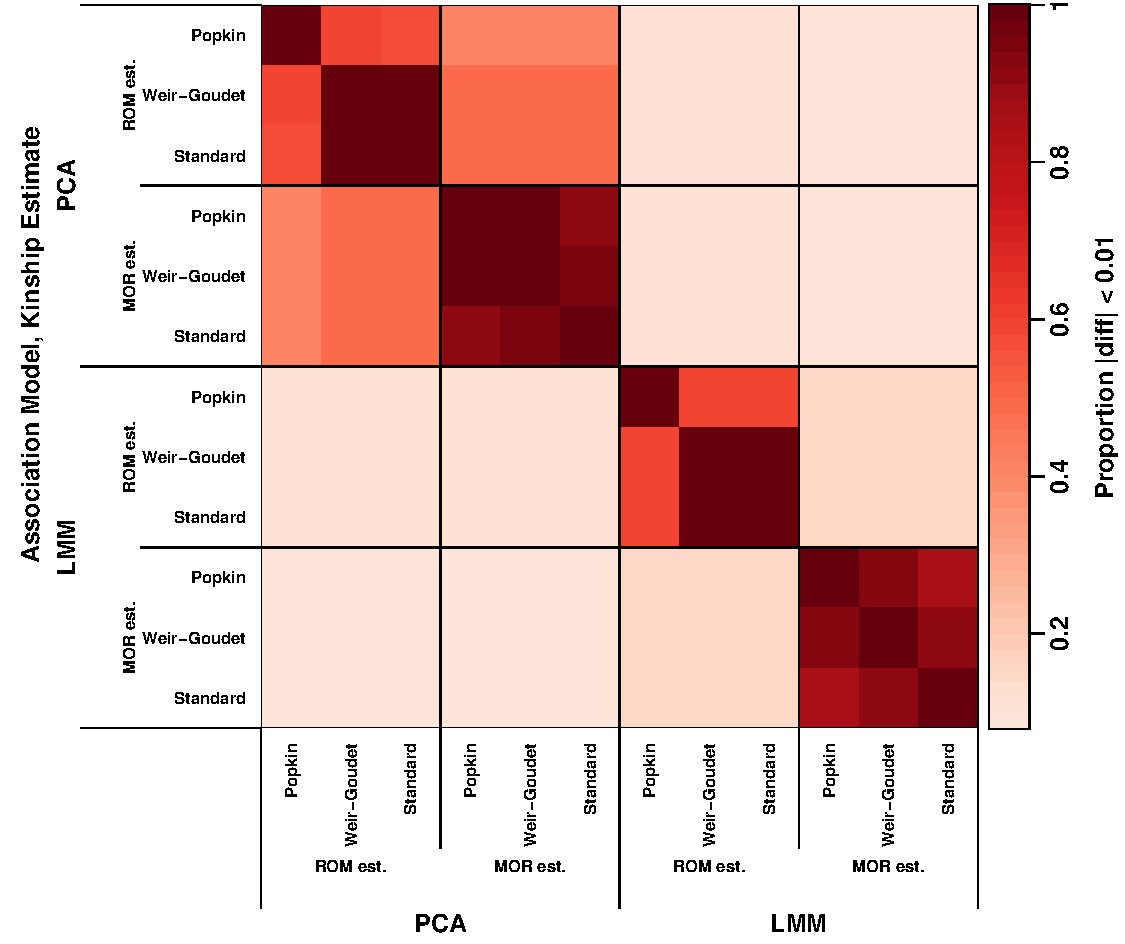
\includegraphics[width=\textwidth]{tgp-nygc-autosomes_ld_prune_1000kb_0.3_maf-0.01/pvals_eq.pdf}
  \caption{
    {\bf Approximate agreement between p-values on 1000 Genomes.}
    See \cref{fig:pvals_eq_sim} for more details.
  }
  \label{fig:pvals_eq_real}
\end{figure}



\end{document}
